\chapter{\Large Introduction}
\label{introchap}

%%%%%%%%%%%%%%%%%%%%%%%%%%%%%%%%%%%%%%%%%%%%
%%%%%%%%%%%%%%%%%%%%%%%%%%%%%%%%%%%%%%%%%%%%
%%%%%%%%%%%%%%%%%%%%%%%%%%%%%%%%%%%%%%%%%%%%
%%%%%%%%%%%%%%%%%%%%%%%%%%%%%%%%%%%%%%%%%%%%
%						Introduction								%
%%%%%%%%%%%%%%%%%%%%%%%%%%%%%%%%%%%%%%%%%%%%
%%%%%%%%%%%%%%%%%%%%%%%%%%%%%%%%%%%%%%%%%%%%
%%%%%%%%%%%%%%%%%%%%%%%%%%%%%%%%%%%%%%%%%%%%
%%%%%%%%%%%%%%%%%%%%%%%%%%%%%%%%%%%%%%%%%%%%

Large scale systems consisting of many interacting subsystems are increasingly common, with applications such as computer networks, smart grids, and robotic sensor networks. The objectives for these applications are often complex; even centralized methods must make tradeoffs between performance and speed in order to optimize these non-convex, nonlinear systems. However, due to inherent limitations in computation, communication, or sensing, large multi-agent systems are often controlled in a distributed fashion. Here, individual agents, or subsystems, must make decisions based on local, often incomplete information, potentially exacerbating tradeoffs between performance and speed. Furthermore, the distributed nature of these multi-agent systems may introduce vulnerabilities to adversarial manipulation: by influencing small subsets of agents, a malicious agent may be able to degrade a system's overall performance.
The overarching goals of this dissertation are to (1) characterize tradeoffs between speed, performance, vulnerability, and information available to agents in distributed control systems, and (2) design algorithms with desirable guarantees in these aspects. 
In order to address these goals, we focus specifically on the following questions:


%%%%%%%%%%%%%%%%%%%%%%%%%%%%%%%%%%%%%%%%%%%%
%%%%%%%%%%%%%%%%%%%%%%%%%%%%%%%%%%%%%%%%%%%%
%%%%%%%%%%%%%%%%%%%%%%%%%%%%%%%%%%%%%%%%%%%%
%%%%%%%%%%%%%%%%%%%%%%%%%%%%%%%%%%%%%%%%%%%%
%						Research Questions							%
%%%%%%%%%%%%%%%%%%%%%%%%%%%%%%%%%%%%%%%%%%%%
%%%%%%%%%%%%%%%%%%%%%%%%%%%%%%%%%%%%%%%%%%%%
%%%%%%%%%%%%%%%%%%%%%%%%%%%%%%%%%%%%%%%%%%%%
%%%%%%%%%%%%%%%%%%%%%%%%%%%%%%%%%%%%%%%%%%%%

\begin{itemize}[leftmargin=*]
\item \textbf{When is fast convergence to near-optimal behavior possible in a distributed system?} (Chapter~\ref{ch2})
\item\textbf{Can agents in a distributed system learn near-optimal correlated behavior despite severely limited information about one another's behavior?} (Chapter~\ref{ch3})
\item\textbf{How does the structure of agent interaction impact the system's vulnerability to adversarial manipulation?} (Chapter~\ref{ch4})
\end{itemize}

This dissertation focuses on game theoretic methods of distributed control, which provide a framework for prescribing agents' control laws in a distributed control system \cite{Marden2008, Zhu2009, Goto2010, Staudigl2012, Fox2010, Lasaulce2011, Alpcan2010, Han2012, MacKenzie2006, Menache2011}. We begin by providing an informal background on game theoretic distributed control, and then we informally state the contributions of this thesis, as prompted by the three research questions above. This informal discussion will be followed by a formal development of necessary background materials, and then a formal summary of  contributions. 

%%%%%%%%%%%%%%%%%%%%%%%%%%%%%%%%%%%%%%%%%%%%
%%%%%%%%%%%%%%%%%%%%%%%%%%%%%%%%%%%%%%%%%%%%
%%%%%%%%%%%%%%%%%%%%%%%%%%%%%%%%%%%%%%%%%%%%
%%%%%%%%%%%%%%%%%%%%%%%%%%%%%%%%%%%%%%%%%%%%
%						Informal GT background    						%
%%%%%%%%%%%%%%%%%%%%%%%%%%%%%%%%%%%%%%%%%%%%
%%%%%%%%%%%%%%%%%%%%%%%%%%%%%%%%%%%%%%%%%%%%
%%%%%%%%%%%%%%%%%%%%%%%%%%%%%%%%%%%%%%%%%%%%
%%%%%%%%%%%%%%%%%%%%%%%%%%%%%%%%%%%%%%%%%%%%

\subsection{Background: Game theoretic distributed control}

Agents' control laws are a crucial component of any multi-agent system. They dictate how individual agents process locally available information to make decisions. Factors that determine the quality of a control law include informational dependencies, asymptotic performance guarantees, convergence rates, and resilience to adversarial influence.

In a game theoretic control law, each agent is assigned a {\it utility function}\footnote{The terms ``utility" and ``payoff" will refer to individual agents' utility functions, whereas ``objective" or ``welfare" will refer to the system level objective function. Note that in the social sciences literature, ``welfare" often refers to the sum of agents' utilities; in this dissertation the term will be used more broadly. By design, maximization of the global objective function will often coincide with maximization of the sum of agents' utilities. } and a {\it learning rule}.\footnote{The terms ``learning rule," ``revision strategy," and ``decision making strategy" will all refer to individual agents' learning rules.} Significant research has been directed at deriving distributed utility functions and learning rules that possess desirable performance guarantees and enable agents to make decisions based on limited information.


\noindent{\it \emph{Utility functions: what should agents optimize?} } 

An agent's local utility function dictates {\it what} it should seek to optimize. Well-studied utility functions from the literature include {\it marginal contribution} \cite{wolpert}, {\it equal share} \cite{marden paper}, and {\it Shapley value} \cite{shapley paper} utilities. Effective utility functions are aligned with the global objective function. This means that when the system is near a globally optimal configuration, individual agents are also performing well with respect to their local utility functions.  An agent's individual utility function typically depends on its own action and on available information about other agents' actions. This interdependence is desirable because an agent's best action with respect to the global objective often depends on the behavior of others. For example, if a subset of agents fails, the remaining agents should compensate accordingly; interdependent utility functions can enable this.

However, interdependence in agents' utility functions adds complexity to the distributed optimization problem. Individual agents do not have full control over the functions they seek to optimize. This can often lead to the emergence of undesirable equilibria when agents simply respond optimally to others' actions. Example~\ref{e:interdependent utilities} demonstrates a simple situation where undesirable equilibria can emerge when agents simply choose the optimal action, conditioned on others' actions. The emergence of inefficient equilibria motivates the study of alternative decision making rules which can act as methods for selecting desired equilibria.

\begin{example}\label{e:interdependent utilities}
Suppose we have two agents, {\it agent 1} and {\it agent 2}. Each agent can perform one of two tasks, {\it task 1}, which has a value of 10, or {\it task 2}, which has a value of 1.  The two agents can observe each other's behavior, but cannot communicate to coordinate their actions. Suppose that the agents can accomplish either task by working together on it, but they cannot accomplish either if they miscoordinate. This scenario is depicted in Figure~\ref{t:simple coordination}.

Because the agents can observe each other's actions, they have sufficient information to evaluate the global objective function. Hence we can simply assign agents' utilities to equal the global objective.\footnote{Assigning utilities equal to the global welfare is often impossible when agents do not have access to global information about others' actions.} Even in this simple situation, where agents have global knowledge of the system objective function and their utilities are exactly equal, inefficient Nash equilibria can emerge.

Informally, in a Nash equilibrium, no agent can improve its utility via a unilateral change of action. In this example, there are two Nash equilibria: an {\it efficient}, or welfare maximizing, equilibrium when the two agents coordinate on task 1, and another {\it inefficient}, or suboptimal, equilibrium when the two agents coordinate on task 2. When agents simply optimize their utilities given others' behavior, they may settle on either an inefficient or an efficient equilibrium. Furthermore, the performance loss associated with inefficient equilibria, is not necessarily bounded. In this example, the difference in value between task 1 and task 2 could be very large, but collaboration on the less valuable task would remain a Nash equilibrium and a possible rest point of a simple utility maximization strategy.



\begin{figure}
\begin{center}
\begin{tabular}{rr|c|c|}
\multicolumn{1}{c}{}&\multicolumn{3}{c}{\textbf{\underline{System objective}}}\\
\multicolumn{2}{r}{}&\multicolumn{2}{c}{\textbf{agent 2}}\\
\multicolumn{2}{r}{}
 &  \multicolumn{1}{c}{task 1}
 & \multicolumn{1}{c}{task 2} \\
\cline{3-4}
\multirow{2}{*}{\textbf{agent 1}}
&task 1 & 10 & 0 \\
\cline{3-4}
&task 2 & 0 & 1 \\
\cline{3-4}
\end{tabular}\quad\quad\quad
\begin{tabular}{rr|c|c|}
\multicolumn{1}{c}{}&\multicolumn{3}{c}{\textbf{\underline{Agent utilities}}}\\
\multicolumn{2}{r}{}&\multicolumn{2}{c}{\textbf{agent 2}}\\
\multicolumn{2}{r}{}
 &  \multicolumn{1}{c}{task 1}
 & \multicolumn{1}{c}{task 2} \\
\cline{3-4}
\multirow{2}{*}{\textbf{agent 1}}
&task 1 & \cellcolor[gray]{0.8}10,10 & 0,0 \\
\cline{3-4}
&task 2 & 0,0 & \cellcolor[gray]{0.8}1,1 \\
\cline{3-4}
\end{tabular}
\end{center}
\caption{A simple coordination task, with the system objective function on the left, and a possible choice of agent utilities on the right. Here, the goal is to design agents' utilities so that they coordinate to accomplish a task. Task 1 is more desirable than task 2. The shaded boxes represent Nash equilibria: neither agent can improve its utility via a unilateral change of action. Coordination on task 2 does not maximize the overall objective or agents' utilities, and is known as an {\it inefficient Nash equilibrium.} One objective in designing effective agent learning rules is to select Nash equilibrium which also maximizes the objective, namely coordination on task 1.}
\label{t:simple coordination}
\end{figure}

\FloatBarrier
\end{example}



\noindent{\it \emph{Learning rules: how should agents optimize?}} 

An agent's learning rule dictate {\it how} it should optimize its utility function. In some cases, it may suffice for each agent to choose the action which maximizes its utility function, given others' current behavior. This is know as a {\it best response} learning rule. However, in many distributed systems, this approach can lead to undesirable equilibria, as shown in Example~\ref{e:interdependent utilities}. Alternative learning rules, such as log-linear learning \cite{Blume1993}, regret matching \cite{blah}, or fictitious play \cite{blah}, have been studied in the literature. \todo{cite some learning rules here}. Noisy best response learning rules can often lead agents toward a global objective optimizer in distributed control systems. Here, agents optimize their utilities most of the time, but occasionally make suboptimal choices. These types of learning rules will be the focus of this dissertation.

The combination of agents' utility functions and learning rules dictates system dynamics, and hence determines both (1) performance with respect to the system level objective, and (2) speed of convergence. Furthermore, agents' ability to evaluate their utility functions depends on locally available information. Thus, information available to agents also impacts system dynamics, and becomes a potential source for vulnerability.


%%%%%%%%%%%%%%%%%%%%%%%%%%%%%%%%%%%%%%%%%%%%
%%%%%%%%%%%%%%%%%%%%%%%%%%%%%%%%%%%%%%%%%%%%
%%%%%%%%%%%%%%%%%%%%%%%%%%%%%%%%%%%%%%%%%%%%
%%%%%%%%%%%%%%%%%%%%%%%%%%%%%%%%%%%%%%%%%%%%
%						Informal statement of contributions				%
%%%%%%%%%%%%%%%%%%%%%%%%%%%%%%%%%%%%%%%%%%%%
%%%%%%%%%%%%%%%%%%%%%%%%%%%%%%%%%%%%%%%%%%%%
%%%%%%%%%%%%%%%%%%%%%%%%%%%%%%%%%%%%%%%%%%%%
%%%%%%%%%%%%%%%%%%%%%%%%%%%%%%%%%%%%%%%%%%%%

\section{Informal statement of contributions}


The following informally summarizes this dissertation's primary contributions in the area of game theoretic distributed control, with respect to the three research questions posed above.

\noindent{\it\emph{Research question \#1: When is fast convergence to near-optimal collective behavior possible in a distributed system? }}

\smallskip

\noindent \textbf{Contribution: Fast convergence to near-optimal collective behavior is possible when agents revise their actions according a a mild variant of log-linear learning, provided (1) agents' utilities are their marginal contribution to the system level objective, and (2) heterogeneity among agents is limited.}


\todo[inline]{check research questions for consistency}

One well-studied method of optimizing behavior in a multi-agent system is to assign agent utilities to be their {\it marginal contribution} to the overall system objective \cite{Wolpert1999}, and have agents make decisions according to the {\it log-linear learning} rule \cite{Blume1993}. In log-linear learning, agents primarily choose utility maximizing actions, but choose suboptimally with a small probability that decreases exponentially with respect to the associated payoff loss. In the long run, marginal contribution utilities with log-linear learning dynamics spends the majority of time at the global objective function maximizer. Unfortunately, worst-case convergence times for log-linear learning are known to be exponential in the number of agents, \cite{Shah2010} often rendering this game theoretic control method impractical for large-scale distributed systems. 

However, when system heterogeneity is limited, i.e., agents can be grouped into a small number of populations according to their action sets and impact on the objective function, a variant of log-linear learning achieves improved worst-case convergence times. In Chapter~\ref{ch2}, we build on the work of \cite{Shah2010} to derive this variant, which converges in near-linear time with respect to the number of agents. 

\noindent{\it \emph{Research question: Can agents learn near-optimal correlated behavior despite severely limited information about one another's behavior? }}

\smallskip

\noindent\textbf{Contribution: Following the algorithm in Chapter~\ref{ch3}, agents with limited knowledge of each other's behavior can learn a utility-maximizing correlated equilibrium.}


Significant research has been directed at deriving distributed learning rules that possess desirable asymptotic performance guarantees and convergence rates and enable agents to make decisions based on limited information. The majority of this research has focused on attaining convergence to (pure) Nash equilibria under stringent information conditions \cite{Young2009, Frihauf2012, Foster2006, Boussaton2012, Poveda2013, Gharesifard2012}. Recently, the research focus has shifted to ensuring convergence to alternate types of equilibria that often yield more efficient behavior than Nash equilibria.  In particular, results have emerged that guarantee convergence to Pareto efficient Nash equilibria \cite{Marden2009,Pradelski2012}, potential function maximizers \cite{Blume1993, Marden2012}, welfare maximizing action profiles \cite{Marden2011, Arieli2012}, and the set of correlated equilibria \cite{Hart2000,Marden2013c,Aumann1987,Foster1997}, among others.  

In most cases highlighted above, the derived algorithms guarantee (probabilistic) convergence to the specified equilibria.  However, the class of correlated equilibria has posed significant challenges with regards to this goal. Learning algorithms that converge to an efficient correlated equilibrium are desirable because optimal system behavior can often be characterized by a correlated equilibrium. Unfortunately, the aforementioned learning algorithms, such as regret matching \cite{Hart2000}, merely converge to the \emph{set} of correlated equilibria. This means that the long run behavior does not necessarily constitute a specific correlated equilibrium at any instance of time.


In Chapter~\ref{ch3} we design and analyze an algorithm that converges to a payoff maximizing coarse correlated equilibrium when agents have no knowledge of others' behavior. Here, agents' utilities depend on collective behavior, but they have no way of evaluating the utility of alternative actions. Our algorithm uses a common random signal as a coordinating entity to eventually drive agents toward the desired collective behavior. In the long run, day to day behavior is selected probabilistically according to the payoff maximizing coarse correlated equilibrium.

\todo[inline]{change I's to we's? at least make it consistent}
 
\noindent{\it \emph{Research question: How does the structure of agent interaction impact a distributed system's vulnerability to adversarial manipulation?}}

\smallskip

 \noindent\textbf{Contribution: If every subset of agent interacts with sufficiently many other agents, the system is more resilient to adversarial manipulation.}


Agents in a distributed system often interact and share information according to a network. The structure of this network not only has an impact on a distributed control algorithm's performance and speed, but also on its resilience to adversarial manipulation. A loosely connected network may be easier to influence, because an adversary may be able to more easily manipulate the information available to subsets of agents, thereby creating impacts that cascade throughout the system. On the other hand, a well-connected network may be more difficult to influence in this way. In Chapter~\ref{ch4}, we investigate such vulnerabilities for  {\it graphical coordination games} \cite{Ullmann1977,Cooper1999} with agents revising their actions according to log-linear learning. Here, we provided a condition based on network structure which guarantees resilience in a graphical coordination game. 

%%%%%%%%%%%%%%%%%%%%%%%%%%%%%%%%%%%%%%%%%%%%
%%%%%%%%%%%%%%%%%%%%%%%%%%%%%%%%%%%%%%%%%%%%
%%%%%%%%%%%%%%%%%%%%%%%%%%%%%%%%%%%%%%%%%%%%
%%%%%%%%%%%%%%%%%%%%%%%%%%%%%%%%%%%%%%%%%%%%
%						Technical Preliminaries						%
%%%%%%%%%%%%%%%%%%%%%%%%%%%%%%%%%%%%%%%%%%%%
%%%%%%%%%%%%%%%%%%%%%%%%%%%%%%%%%%%%%%%%%%%%
%%%%%%%%%%%%%%%%%%%%%%%%%%%%%%%%%%%%%%%%%%%%
%%%%%%%%%%%%%%%%%%%%%%%%%%%%%%%%%%%%%%%%%%%%



\section{Technical Preliminaries}

In this section, we provide technical motivation for the study of game theoretic control algorithms, and we also establish the technical background and notation necessary to formally state the main contributions of this dissertation.

Consider a multi-agent system consisting of agents, $N = \{1,2,\ldots,n\}$, where each agent $i\in N$ has a finite action set, $A_i$. The set of joint actions will be denoted by $\mathcal{A} = \prod_{i\in N} A_i$,  and a joint action will be written as $$a = (a_1,a_2,\ldots,a_n)\in\mathcal{A},$$ or using the shorthand notation $$(a_i,a_{-i}) := (a_1,a_2,\ldots,a_i,\ldots,a_n)\in\mathcal{A}.$$ 


Suppose we aim to design agents' local control laws in order to maximize the global objective function, $W:\mathcal{A}\to \mathbb{R}.$ Here, an agent's control law will be defined by a {\it utility function} and {\it learning rule}.


\subsection{Agent utility functions}


Each agent, $i\in N$, is assigned a utility function, $U_i: \mathcal{A}\to\mathbb{R},$ which maps each joint action to a value in $\R.$  When agents' information about others' actions is more limited, utilities can be designed accordingly, e.g., taking the form $U_i:\prod_{j\in N_i\cup \{i\}}A_j\to \R,$ where $N_i$ represents the set of agent $i$'s neighbors, as defined by some underlying communication graph. Alternatively, agent utilities may also incorporate additional information about an underlying system state, e.g., $U_i:\mathcal{A}\times X\to \R$, where $X$ represents a set of possible states of the surrounding environment.

We have now formally defined all the elements of a game.

\begin{defn}
A {\it game} is a tuple $(N,\{A_i\}_{i\in N}, \{U_i\}_{i\in N})$ consisting of a set of agents, $N$, and their associated action sets, $\{A_i\}_{i\in N}$, and utility functions, $\{U_i\}_{i\in N}$.
\end{defn}

Prior to defining dynamics over a game, $G$, we often view the Nash equilibrium as a natural rest point, since it occurs when no agent can improve its utility by unilaterally changing its action.

\begin{defn}
For a game $G = \left(N,\{A_i\}_{i\in N},\{U_i\}_{i\in N}\right),$ action profile $a = (a_i,a_{-i})\in \mathcal{A}$ is a {\it Nash equilibrium} \cite{add citation} if it satisfies:
$$U_i(a)\geq U_i(a_i^\prime,a_{-i}),\quad \forall i\in N, a_i^\prime\in A_i$$
\end{defn}


Commonly studied utility functions include marginal contribution \cite{Wolpert1999}, equal share \cite{blah}, and Shapley value \cite{blah} utilities. In this dissertation, we focus primarily on marginal contribution utilities, as defined below.\footnote{Utility design is a widely studied area in game theory \cite{blah}, and is not a topic of this thesis. We employ well-studied utility functions which are suitable for our distributed optimization purposes, and focus our study on agents' learning rules and communication structure.} 



\begin{defn}
An agent's {\it marginal contribution}\cite{Wolpert1999} to the system objective, $W:\mathcal{A}\to \R$, corresponding to joint action $a = (a_i,a_{-i})\in \mathcal{A}$ is defined by:
$${\rm MC}_i(a) = W(a) - W(\emptyset,a_{-i}),$$
where $(\emptyset,a_{-i})$ represents removing agent $i$ from the system, while keeping other agents fixed at actions $a_{-i}.$
\end{defn}

Assigning agents' utilities to be their marginal contribution to the system welfare ensures that the optimal allocation corresponds to a Nash equilibrium. Furthermore, this choice of utility function defines a potential game.

\begin{defn}
A game $(N,\{A_i\}_{i\in N}, \{U_i\}_{i\in N})$ is a {\it potential game}\cite{Monderer1996} if there exists a potential function, $\phi:\mathcal{A}\to \R$ satisfying
$$\phi(a_i,a_{-i}) - \phi(a_i^\prime,a_{-i}) = U_i(a_i,a_{-i}) - U_i(a_i^\prime,a_{-i})$$
for all $i\in N,$ all $(a_i,a_{-i})\in \mathcal{A},$ and all $a_i^\prime\in A_i.$
\end{defn}

In fact, assigning agents' utilities to be their marginal contribution to the system objective defines a potential game with $\phi(a) = W(a),\,\forall a\in \mathcal{A},$ i.e., the potential function is equal to the system welfare function. This is useful, because there exist well studied learning algorithms which converge to a potential function maximizer, e.g., log-linear learning \cite{Blume1993}, which we will discuss in detail in Section~\ref{s:learning rules}. 


Finally, marginal contribution utilities can also reduce informational requirements in certain classes of distribution control problems, as we show in  Example~\ref{e:resource allocation}.

\begin{example}
Consider a {\it resource allocation} task, where we wish to allocate agents in $N = \{1,2,\ldots, n\}$ to a set of resources $R = \{r_1,r_2,\ldots,r_n\}$. Here, agent's action sets are a collection of subsets of $R$, i.e., $A_i\subseteq 2^R,$ so that an action $a_i\in A_i$ represents allocation of agent $i$ to subset $a_i\subseteq R.$

In resource allocation problems, the global welfare depends on the welfare attained at each resource. Typically, resource allocation problems have a {\it separable welfare function}:
$$W_{\rm global}(a) = \sum_{r\in R} W_r(\{a\}_r),\quad a\in\mathcal{A},$$
where $W_r$ is the welfare function associated with resource $r\in R$, and $\{a\}_r$ represents the set of agents selecting resource $r$ in action profile $a$. 

It is straightforward to show that, when the global welfare function is separable, an agent's marginal contribution can be written as
$$MC_i(a_i,a_{-i}) = \sum_{r\in a_i}W_r\left(\{a\}_r\right) - W_r\left(\{a\}_r\setminus\{i\}\right).$$
Hence, agent $i$ only needs information about other agents allocated to resources $r\in a_i\subseteq R$ to evaluate its marginal contribution.
\end{example}


\subsection{Learning rules}

Agents' learning rules are the second component of a game theoretic control law. Learning rules dictate how agents process information in order to optimize their utility functions. Formally, the game $G$ is repeated over time, producing a sequence of joint actions, $a(0), a(1),a(2),\ldots.$ At each time $t\in\N$, some subset of agents, $S\subseteq N$ has the opportunity to revise their actions independently according to a learning rule of the form:
$$a_i(t) = \Pi_i(\{a(\tau)\}_{\tau=0,1,\ldots,t-1};U_i(\cdot)$$
which may depend on the history of agents' joint actions, and on the form of agent $i$'s utility function. The precise form of a learning rule can vary, depending on the information available to agent $i$ at time $t$. For example, a learning rule may instead be based on a finite history of joint actions, or on estimated (rather than exact) information.

For concreteness, we now provide two well studied learning rules: the {\it best response learning rule} and the {\it log-linear learning rule}.

\begin{defn}
Given a game $G = \left(N,\{A_i\}_{i\in N},\{U_i\}_{i\in N}\right)$, and an initial joint action $a(0)\in \mathcal{A},$ the {\it best response learning rule} proceeds by repeating the following steps at each time $t\in \N$:
\begin{enumerate}
    \item Select an agent $i\in N$ uniformly at random.\footnote{Although selecting an agent uniformly at random is a centralized task, it is possible to define a fully decentralized learning rule in which agents update their actions in continuous time according to arrival times associated with independent Poisson processes. In Chapter~\ref{ch2} we formally define such a learning rule, but here we restrict ourselves to discrete-time learning rules for simplicity.}
    \item Agent $i$ selects a ``best response" action, i.e., agent $i$ selects action
    $$a_i\in \argmax_{a_i^\prime\in A_i}U_i(a_i^\prime,a_{-i}),$$
    which maximizes its utility, given all other agents' current actions.
    \item The ensuing joint action at time $t+1$ is 
    $$a(t+1) = (a_i,a_{-i}(t)),$$ i.e., agent $i$ plays its best response action, and all other agents repeat their previous actions.
\end{enumerate}
\end{defn}

In potential games, the best response learning rule converges to a Nash equilibrium of the game. However, this Nash equilibrium need not be efficient. For example, recall the game defined in Example~\ref{e:interdependent utilities}, with the system welfare and agent utility functions below.

%\begin{figure}
\begin{center}
\begin{tabular}{rr|c|c|}
\multicolumn{1}{c}{}&\multicolumn{3}{c}{\textbf{\underline{System objective}}}\\
\multicolumn{2}{r}{}&\multicolumn{2}{c}{\textbf{agent 2}}\\
\multicolumn{2}{r}{}
 &  \multicolumn{1}{c}{task 1}
 & \multicolumn{1}{c}{task 2} \\
\cline{3-4}
\multirow{2}{*}{\textbf{agent 1}}
&task 1 & 10 & 0 \\
\cline{3-4}
&task 2 & 0 & 1 \\
\cline{3-4}
\end{tabular}\quad\quad\quad
\begin{tabular}{rr|c|c|}
\multicolumn{1}{c}{}&\multicolumn{3}{c}{\textbf{\underline{Agent utilities}}}\\
\multicolumn{2}{r}{}&\multicolumn{2}{c}{\textbf{agent 2}}\\
\multicolumn{2}{r}{}
 &  \multicolumn{1}{c}{task 1}
 & \multicolumn{1}{c}{task 2} \\
\cline{3-4}
\multirow{2}{*}{\textbf{agent 1}}
&task 1 & \cellcolor[gray]{0.8}10,10 & 0,0 \\
\cline{3-4}
&task 2 & 0,0 & \cellcolor[gray]{0.8}1,1 \\
\cline{3-4}
\end{tabular}
\end{center}
%\end{figure}
\medskip

Indeed, this example is a potential game agent utilities defined by their marginal contribution to the system welfare, and potential function equal to the system objective. Here, the best response process will converge to one of the two Nash equilibria shaded in grey, depending on the initial joint action, $a(0),$ and on which agent is selected to update at each time. Hence, there is no guarantee that the best response process will select a welfare-optimizing Nash equilibrium.



Mathematically, the best response process defines a Markov chain over the joint action space. The Markov chain associated with the best response learning rule for the example above is shown in Figure~\ref{f:BR_MarkovChain}. This Markov chain has two stationary distributions,
$$\pi_1 = \begin{bmatrix} 1&0&0&0 \end{bmatrix},
\quad
\text{and}
\quad 
\pi_2 = \begin{bmatrix} 0&0&0&1\end{bmatrix},$$
where the four joint actions are in the order shown in Figure~\ref{f:BR_MarkovChain}.
With respect to the global objective function, $\pi_1$ is optimal, whereas $\pi_2$ is suboptimal. 

\begin{figure}
    \centering
    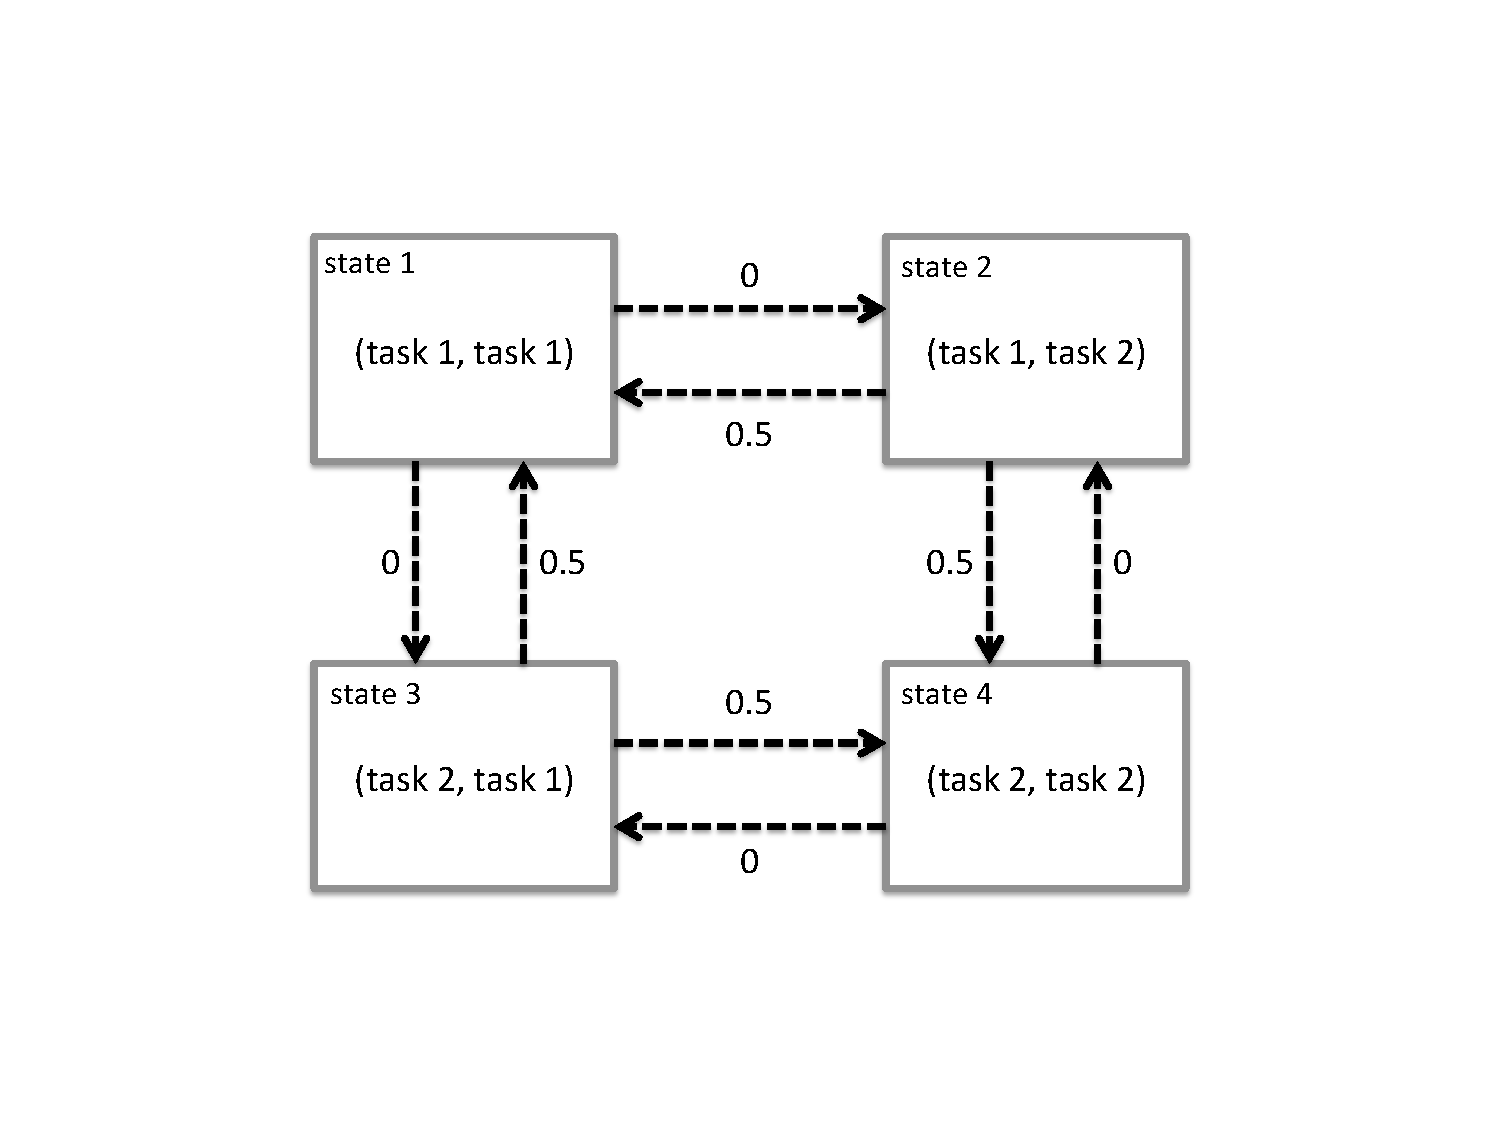
\includegraphics[scale=0.35, clip, trim=15mm 15mm 15mm 15mm]{BR_MarkovChain}
    \caption{Underlying Markov chain corresponding to the best response process over the game in Example~\ref{e:interdependent utilities}}
    \label{f:BR_MarkovChain}
\end{figure}

Log-linear learning belongs to the class of perturbed best response learning rules: here, an updating agent selects a best response action the majority of the time, but occasionally selects suboptimally. As we will show, log-linear learning acts as a method for selecting one of the (possibly many) stationary distributions of a best response process.

\begin{defn}
Given a game $G = \left(N,\{A_i\}_{i\in N}, \{U_i\}_{i\in N}\right)$, and an initial joint action $a(0)\in\mathcal{A},$ the {\it log-linear learning rule} proceeds by repeating the following steps at each time $t\in \N:$
\begin{enumerate}
    \item Select an agent $i\in N$ uniformly at random.
    \item Agent $i$ selects an action probabilistically, according to:
    $$\Pr[a_i(t+1) = a_i] = {\exp\left(\beta U_i(a_i,a_{-i}(t)\right)\over
    \sum_{a_i^\prime\in A_i} \exp\left(\beta U_i(a_i^\prime,a_{-i}(t)\right)}$$ where $\beta$ is a design parameter.
    \item The ensuing joint action at time $t+1$ is $$a(t+1) = \left(a_i(t+1),a_{-i}(t)\right).$$
\end{enumerate}

\end{defn}

In log-linear learning, as parameter $\beta\to\infty$, an updating agent chooses a utility maximizing action with higher probability. As $\beta\to 0,$ an updating agent chooses uniformly at random. 







\todo[inline]{find a good place for the notation summary}
\begin{figure}
\vspace{.15in}
\begin{mdframed}
\underline{\textbf{Notation and Terminology}}
\begin{itemize}
    \item $N = \{1,2,\ldots,n\}$ - set of agents
    \item $A_i$ - agent $i$'s finite action set
    \item $\mathcal{A}:=\prod_{i\in N} A_i$ - the joint action space
    \item $a = (a_1,a_2,\ldots a_i,\ldots,a_n) = (a_i,a_{-i})\in\mathcal{A}$ - a joint action
    \item $W:\mathcal{A}\to\R$ - the system objective function. Also referred to as the system welfare function.
    \item $U_i:\mathcal{A}\to\R$ - agent $i$'s utility function
    \item ${\rm MC}_i(a)$ - agent $i$'s marginal contribution to the system objective at joint action $a\in \mathcal{A}$
    \item Best response learning rule - a decision making rule in which the updating agent selects a utility maximizing action, given other agents' current actions
    \item Log-linear learning rule - a decision making rule in which the updating agent selects a utility maximizing action with high probability, and selects a suboptimal action with a probability that decreases exponentially with respect to the associated payoff loss.
\end{itemize}
\end{mdframed}
\end{figure}



%\begin{enumerate}
%    \item the setting: a distributed control system. agents, actions, objective function
%    \item Our approach: game theoretic control
%    \begin{enumerate}
%        \item Utility function that maps local information to a utility/payoff. Give a small preview of the types of utility function we use. Appropriate design varies depending on the application. My focus was on learning algorithms, so typically I assigned utilities that made analysis simple in order to gain intuition about the question I was trying to ask. Not sure whether to say this or how to convey it....
%        \item Learning rule that dictates agents' decisions. Our focus is on probabilistic learning rules. Reference Markov chains section in the appendix. Discrete time, so this yields a sequence of joint actions $a(0),a(1),\ldots.$ Small discussion that these are random variables, perhaps. Include an example (LLL) and state that the majority of the dissertation will focus on LLL, with the exception of the CCE work.
%    \end{enumerate}
%    \item Goal (in general): design utilities and learning rules with desired performance
%    \begin{enumerate}
%        \item Desired long run performance. Given parameter $\varepsilon>0$, should be able to tune learning algorithm parameters to achieve:
%        $$\lim_{t\to\infty}\mathbb{E}[ W(a(t)]\geq \max_{a\in\mathcal{A}}W(a) - \varepsilon$$
%        \item Fast convergence rates. Given $\delta > \varepsilon$, desired
%        $$\mathbb{E}[W(a(t))]\geq \max_{a\in\mathcal{A}}W(a) - \delta$$
%        for all $t\geq T$, for some ``reasonable" convergence time $T$. Discussion here that $T$ typically depends on the number of agents, action sets, etc., and can often be exponential in these parameters. Goal here is to design a learning rule that's linear. Reference an example and log-linear learning.
%        \item Resilience to adversaries. Suppose an adversary is able to manipulate information available to small subsets of agents. Is it possible for limited info manipulation to cascade and create catastrophic performance failures? Goal is for it not to be.
%    \end{enumerate}
%\end{enumerate}
%
%
%%%%%%%%%%%%%%%%%%%%%%%%%%%%%%%%%%%%%%%%%%%%%
%%%%%%%%%%%%%%%%%%%%%%%%%%%%%%%%%%%%%%%%%%%%%
%%%%%%%%%%%%%%%%%%%%%%%%%%%%%%%%%%%%%%%%%%%%%
%%%%%%%%%%%%%%%%%%%%%%%%%%%%%%%%%%%%%%%%%%%%%
%%						Formal statement of contributions				%
%%%%%%%%%%%%%%%%%%%%%%%%%%%%%%%%%%%%%%%%%%%%%
%%%%%%%%%%%%%%%%%%%%%%%%%%%%%%%%%%%%%%%%%%%%%
%%%%%%%%%%%%%%%%%%%%%%%%%%%%%%%%%%%%%%%%%%%%%
%%%%%%%%%%%%%%%%%%%%%%%%%%%%%%%%%%%%%%%%%%%%%
%
%\section{Formal statement of contributions}
%
%Relate to the goals above. State each main theorem as a contribution here. First a reminder of the three main questions.
%
%\subsection{Fast convergence contributions}
%
%\subsection{CCE contributions}
%
%\subsection{Adversarial vulnerability contributions}
%
%\todo[inline]{Add large ``future work" section. There's a lot left to do!}